\chapter{基准New Keynesian模型}
\label{sec:Basic-NK-model}

\section{家庭部门}
\label{sec:Basic-NK-model-HH-sector}


假定cashless economy,家庭的效用函数$U(C_t, N_t)$表示为\footnote{膏按:RBC(DSGE)在经验研究中中常用工作小时数而非就业人员数作为$N_t$的代理变量,其相关讨论早期文献可见\cite{Hansen:1985ku,Rogerson:1988js};近期的综述见\cite{Rogerson:2009ez}。}
\begin{equation}
  \label{eq:utility-function}
  U(C_t, N_t) = \frac{C_t^{1-\sigma}}{1-\sigma} - \psi \cdot \frac{N_t^{1+\eta}}{1+\eta},
\end{equation}

HH问题。目标:追求效用最大化
\begin{align}
  \label{eq:HH-problem-max}
  \max_{\{C_t, N_t, B_{t+1}\}} & E_0 \sum_{t=0}^{\infty} \beta^t \cdot U(C_t, N_t), \nonumber \\
&st. \quad P_t \cdot C_t + B_{t+1} \le W_t \cdot N_t + Div_t - P_t \cdot T_t + (1+i_{t-1}) \cdot B_t,
\end{align}
其中$Div_t$表示dividends,中间产品企业的(垄断)利润。$T_t$表示税收或转移支付。$i_t$为名义利率。

建Lagrange
\begin{equation}
  \label{eq:HH-problem-lagrange}
  \mathcal{L} = E_0 \sum_{t=0}^{\infty} \beta^t \cdot \{ U(C_t, N_t) + \lambda_t \cdot \left[W_t \cdot N_t + Div_t - P_t \cdot T_t + (1+i_{t-1}) \cdot B_t - P_t \cdot C_t - B_{t+1}\right]\}.
\end{equation}

FOCs
\begin{align*}
  \frac{\partial \mathcal{L}}{\partial C_t}=0 &\Rightarrow C_t^{-\sigma} = \lambda_t \cdot P_t \\
  \frac{\partial \mathcal{L}}{\partial N_t}=0 & \Rightarrow \psi \cdot N_t^{\eta} = \lambda_t \cdot W_t \\
\frac{\partial \mathcal{L}}{\partial B_{t+1}}=0 & \Rightarrow \frac{\partial \{\lambda_t \cdot (1 + i_{t-1}) \cdot B_t\}}{\partial B_{t+1}} - \lambda_t = \frac{\partial \beta \cdot E_t \{ \lambda_{t+1} \cdot (1 + i_{t}) \cdot B_{t+1} \} } {\partial B_{t+1}} - \lambda_t = 0\\
\end{align*}

整理得
\begin{gather}
  \label{HH-FOC-labor-supply}
  \psi \cdot N_t^{\eta} = C_t^{-\sigma} \cdot w_t \\
\label{HH-FOC-euler-consumption}
  C_t^{-\sigma} = \beta \cdot E_t\{ C_{t+1}^{-\sigma} \cdot (1+i_t) \cdot \frac{P_t}{P_{t+1}}\}=\beta \cdot E_t\{ C_{t+1}^{-\sigma} \cdot (1+i_t) \cdot ( 1+\pi_{t+1} )^{-1}\},
\end{gather}
其中$w_t \equiv \frac{W_t}{P_t}$表示实际工资,$\pi_t + 1 \equiv P_t/P_{t-1}$表示通货膨胀率。由  \eqref{HH-FOC-labor-supply}可得Frisch elasticity of labor supply为$1/\eta$\footnote{假定短时期内家庭的总财富(总消费)不变,市场上工资的变化只影响家庭的劳动力供应,Frisch labor supply elasticity\citep{Frisch:1932wk,Frisch:1959jt}可表示为
  \begin{equation*}
    \frac{\partial n_t}{\partial w_t} \cdot \frac{w_t}{n_t},
  \end{equation*}
可参考\cite[pp.279]{Heer:2009ig},以及\cite{Christiano:2010wla}。}。



\section{企业部门}
\label{sec:Basic-NK-model-firm-sector}

\subsection{最终产品生产部门}
\label{sec:Basic-NK-model-final-produc-firm-sector}
最终产品部门以中间产品$Y_t(j), j \in [0,1]$的组合为投入要素,产出$Y_t$,符合完全竞争假定。\cite{Dixit:1977tv}形式的生产规模报酬不变生产函数为
\begin{equation}
  \label{eq:fin-prod-prod-func}
  Y_t = \left[ \int_{0}^{1} Y_t(j)^{\frac{\epsilon - 1}{\epsilon}} dj\right]^{\frac{\epsilon}{\epsilon - 1}},
\end{equation}
其中$\epsilon > 1$表示$j^{th}$中间产品的替代弹性。

最终产品厂商问题:在给定$P_t(j)$的情况下,通过选择$Y_t(j)$的投入追求利润最大化

\begin{equation}
  \label{eq:fin-prod-problem-max}
  \max_{Y_t(j)} P_t \cdot Y_t - \int_{0}^{1} P_t(j) \cdot Y_t(j) dj ,
\end{equation}

引入式\eqref{eq:fin-prod-prod-func},FOC整理可得对$j$中间产品的需求函数
\begin{equation}
  \label{eq:demand-for-intm-j}
  Y_t(j) = \left( \frac{P_t(j)}{P_t}
\right)^{-\epsilon} \cdot Y_t,
\end{equation}

进而根据完全竞争市场假定
\begin{equation*}
  \begin{split}
    P_t \cdot Y_t & \equiv \int_0^1 P_t(j) \cdot Y_t(j) dj \\
    &=\left[\int_0^1 \left(\frac{P_t(j)}{P_t}\right)^{-\epsilon} \cdot Y_t \cdot P_t(j) dj \right] \\
    &=\left[\int_0^1 P_t(j)^{1-\epsilon} dj \right] \cdot P_t^{\epsilon} \cdot Y_t,\\
  \end{split}
\end{equation*}
整理得最终产品价格的决定(aggregate price index):
\begin{equation}
  \label{eq:agg-price-index}
  P_t = \left[
    \int_0^1 P_t(j)^{1-\epsilon} dj
  \right]^{\frac{1}{1-\epsilon}}
\end{equation}

\subsection{中间产品生产部门}
\label{sec:Basic-NK-model-intm-produc-firm-sector}
中间产品生产部门假定处于垄断竞争状态。代表企业$j$雇佣劳动力$N_t(j)$生产$Y_t(j)$,生产函数形式
\begin{equation}
  \label{eq:intm-prodc-func}
  Y_t(j) = A_t \cdot N_t(j),
\end{equation}
其中$A_t$表示外生的生产率冲击,它对所有中间产品生产者都是相同的。对劳动力的总需求为$j$个厂商的加总。
\begin{equation}
  \label{eq:Labor-D-S}
  N_t = \int_0^1 N_t(j)dj.
\end{equation}

\subsubsection{成本最小化:边际成本与工资}
\label{sec:intm-min-cost}
中间产品生产者$j$的问题可以表示为两阶段优化。第一阶段为成本最小化:在给定工资$W_t$的基础上,选择雇佣劳动力投入$N_t(j)$,生产中间品$Y_t(j)$,以满足最终产品生产部门对$Y_t(j)$的需求,
\begin{equation}
  \label{eq:intm-prod-max-N}
  \begin{split}
      \min_{N_t(j)} &W_t \cdot N_t(j),\\
      &st. \quad A_t \cdot N_t(j) \ge \left( \frac{P_t(j)}{P_t}\right)^{-\epsilon} Y_t,
  \end{split}
\end{equation}
第二行LHS和RHS分别表示中间产品$Y_t(j)$的供应和需求,见式\eqref{eq:intm-prodc-func}和式 \eqref{eq:demand-for-intm-j}。

建Lagrange
\begin{equation*}
  \mathcal{L} = W_t \cdot N_t(j) + \lambda_t \cdot \left[
\left(\frac{P_t(j)}{P_t}\right)^{-\epsilon} \cdot Y_t - A_t \cdot N_t(j)
\right],
\end{equation*}
其中拉格朗日乘子$\lambda_t$表示$j$生产额外1单位$Y_t(j)$的影子价格(边际成本),设为$MC_t \equiv \lambda_t $.

FOC:
\begin{equation*}
  MC_t = \frac{W_t}{A_t}
\end{equation*}

或者用实际价格形式表示
\begin{equation}
  \label{eq:intm-prod-min-N-mc}
    mc_t = \frac{MC_t}{P_t} = \frac{W_t}{A_t \cdot P_t} = \frac{w_t}{A_t}.
\end{equation}

式\eqref{eq:intm-prod-min-N-mc}  反映了实际(边际成本)和实际工资的对应关系。

\subsubsection{利润最大化:定价策略}
\label{sec:intm-max-profit}
在此基础上,第二阶段,中间产品生产者$j$对自己的产品$Y_t(j)$定价$P_t(j)$,以追求实际利润$\Pi_t$最大化。
\begin{equation}
  \label{eq:intm-prod-profit}
  \begin{split}
    \Pi_t(j) &= \frac{P_t(j) \cdot Y_t(j)}{P_t} - \frac{W_t \cdot N_t(j)}{P_t} \\
    &=\frac{P_t(j)}{P_t} \cdot Y_t(j) - mc_t \cdot Y_t(j) \\
    &=\left( \frac{P_t(j)}{P_t}\right)^{1-\epsilon} \cdot Y_t - mc_t \cdot \left( \frac{P_t(j)}{P_t}\right)^{-\epsilon} \cdot Y_t
  \end{split}
\end{equation}

粘性价格。在$t$时期,中间产品生产者$j$ 有$\phi<1$的概率不能调整价格,维持上一期的定价$P_{t-1}(j)$;有$1-\phi$的概率可以调整价格,将产品售价更新为$P_t^{\#}(j)$。
\begin{equation}
  \label{eq:intm-stick-prices}
  P_t(j) =
  \begin{cases} P_{t-1}(j) &\mbox{with prob.} \quad \phi \\
    P_t^{\#}(j) & \mbox{else} \quad 1-\phi
\end{cases}
\end{equation}

根据模型假设,中间产品生产部门由于垄断产生的利润$\Pi_t$,流回到家庭部门,供消费以提升效用,满足跨期消费的Euler equation式\eqref{HH-FOC-euler-consumption},设$\tilde{M}_{t+s} \equiv \beta^s \cdot \frac{U_{C,t+s}}{U_{C,t}}$作为discount factor。从$t$期向前直到$t+s$期,$j$不能自由调整价格的概率是$\phi^s$。此外,从$t$期向前直到$t+s$期,$j$不能自由调整价格的概率是$\phi^s$。
由此,$j$生产者forward-looking的随机折旧因子为$\phi^s \cdot \tilde{M}_{t+s}$。

先来看式\eqref{eq:intm-stick-prices}中$p^{\#}_j(j)$的决定。$t$期中间品生产者$j$的利润最大化问题表示为
\begin{equation*}
  \begin{split}
    &\max_{P_t(j)} E_t \sum_{s=0}^{\infty} \phi^s \cdot \tilde{M}_{t+s} \cdot \Pi_{t+s} \\
    &=\max_{P_t(j)} E_t \sum_{s=0}^{\infty} \left(\beta \cdot \phi \right)^s \cdot \frac{U_{C,t+s}}{U_{C,t}} \cdot \left[
      \frac{P_{t+s}(j)}{P_{t+s}} \cdot Y_{t+s}(j) - mc_{t+s} \cdot Y_{t+s}(j)
    \right]\\
    &=\max_{P_t(j)} E_t \sum_{s=0}^{\infty} \left(\beta \cdot \phi \right)^s \cdot \frac{U_{C,t+s}}{U_{C,t}} \cdot Y_{t+s} \cdot
    \left[
      \left( \frac{P_{t}(j)}{P_{t+s}} \right)^{1-\epsilon} - mc_{t+s} \cdot \left( \frac{P_{t}(j)}{P_{t+s}} \right)^{-\epsilon}
    \right],
  \end{split}
\end{equation*}

FOC wrt $P_{t}(j)$,整理得
\begin{equation}
  \label{eq:intm-update-price-principle}
  P_{t}(j) = \frac{\epsilon}{\epsilon -1} \cdot \frac
{
  E_t \sum_{s=0}^{\infty} \left(\beta \cdot \phi \right)^s \cdot U_{C,t+s} \cdot Y_{t+s} \cdot mc_{t+s} \cdot P_{t+s}^{\epsilon}
}
{
  E_t \sum_{s=0}^{\infty} \left(\beta \cdot \phi \right)^s \cdot U_{C,t+s} \cdot Y_{t+s} \cdot P_{t+s}^{\epsilon-1}
}
\end{equation}
式\eqref{eq:intm-update-price-principle} RHS分子和分母均与$j$无关,即在价格粘性的情况下,forward-looking的所有中间产品生产者$j\in[0,1]$,如果有机会调整价格(概率$1-\phi$),都会遵循相同的价格调整策略,设为$P^{\#}_{t} \equiv P^{\#}_{t}(j), \forall j$。上式改写为

\begin{equation}
  \label{eq:intm-update-price-aux}
  P^{\#}_t = \frac{\epsilon}{\epsilon  -1} \cdot \frac{X_{1,t}}{X_{2,t}},
\end{equation}
其中辅助变量
\begin{align}
\label{auxiliary-X1}
  X_{1,t} &\equiv U_{C,t} \cdot Y_t \cdot P_{t}^{\epsilon} \cdot mc_t + \beta \cdot \phi \cdot E_t X_{1,t+1},\\
\label{auxiliary-X2}
  X_{2,t} &\equiv U_{C,t} \cdot Y_t \cdot P_{t}^{\epsilon-1} + \beta \cdot \phi \cdot E_t X_{2,t+1}.
\end{align}

为了让变量平稳,定义$x_{1,t} \equiv X_{1,t}/P_{t}^{\epsilon}$,$x_{2,t} \equiv X_{2,t}/P_{t}^{\epsilon-1}$,式  \eqref{eq:intm-update-price-aux}变为
\begin{equation}
  \label{eq:intm-update-price-aux-stationary}
  P^{\#}_t = \frac{\epsilon}{\epsilon  -1} \cdot \frac{x_{1,t}}{x_{2,t}} \cdot P_t.
\end{equation}

或者定义reset price的通胀项$(1+ \pi^{\#}_t) \equiv P^{\#}_t / P_{t-1}$,将式\eqref{eq:intm-update-price-aux-stationary}由价格形式改写为通货膨胀率的形式
\begin{equation}
  \label{eq:intm-update-inflation-aux}
  (1+\pi^{\#}_t) = \frac{\epsilon}{\epsilon -1} \cdot \left( 1+\pi_t \right) \cdot \frac{x_{1,t}}{x_{2,t}}.
\end{equation}

根据\eqref{eq:intm-update-price-aux-stationary},在flexible price即$\phi =0$的情况下,$\forall j$ 中间产品的定价为$P^{\#}_t = \frac{\epsilon}{\epsilon -1} \cdot (mc_t \cdot P_t)$,即名义的边际成本乘以markup。


\subsection{最终产品定价:Calvo assupmtion}
\label{sec:final-produc-price}

Aggregate price index 式\eqref{eq:agg-price-index}中含有$j$,为了消除中间产品生产者的价格异质性对最终产品价格的影响,引入式\eqref{eq:intm-stick-prices},根据Calvo assumption \citep{Calvo:1983uqa}得
\begin{align}
\label{eq:agg-price-index-noj}
  P_t^{1-\epsilon} &= \int_{0}^1 P_t(j)^{1-\epsilon} dj \nonumber\\
                   &= \int_{0}^{1-\phi} \left(P_t^{\#}\right)^{1-\epsilon} dj + \int_{1-\phi}^1 \left(P_{t-1}(j)\right)^{1-\epsilon} dj\nonumber\\
                   &= \int_{0}^{1-\phi} \left(P_t^{\#}\right)^{1-\epsilon} dj + \int_{0}^{\phi} \left(P_{t-1}(j)\right)^{1-\epsilon} dj\nonumber\\
                   &= (1-\phi) \cdot \int_{0}^{1} \left(P_t^{\#}\right)^{1-\epsilon} dj + \phi \cdot \int_{0}^1 \left(P_{t-1}(j)\right)^{1-\epsilon} dj \nonumber\\
                   &=(1-\phi) \cdot \left(P^{\#}_t\right)^{1-\epsilon} + \phi \cdot \left(P_{t-1}\right)^{1-\epsilon}
\end{align}

或者以reset price inflation形式表示为
\begin{equation}
  \label{eq:agg-inflation-index}
  \left(1+\pi_t\right)^{1-\epsilon} = (1-\phi) \cdot \left(1+\pi^{\#}_t\right)^{1-\epsilon} + \phi
\end{equation}

\section{外生技术冲击}
\label{sec:exo-prod-shock}
设外生技术冲击满足$\log$形式的AR(1)过程
\begin{equation}
  \label{eq:exo-prod-shock}
  \ln A_t = \rho_a \cdot \ln A_{t-1} + \varepsilon_{a,t}
\end{equation}
其中$0<\rho_a<1$,$E\{\varepsilon_{a,t}\}=0$。

\section{总量均衡}
\label{sec:Equilibrium-cond}



\subsection{家庭部门消费的决定}
\label{equilibrium-cond-HH-consumption}
均衡状态下,家庭持有的债券和净转移支付为零,$B_t=T_t = 0$ $\forall t$。$Div_t$来自全部中间产品生产者的垄断利润之和,
\begin{equation}
  \label{eq:quili-cond-HH-Div-Pi}
\begin{split}
  \frac{Div_t}{P_t} &= \frac{\Pi_t}{P_t} \\
  &\equiv \int_{0}^1 \left[ \frac{P_t(j)}{P_t} \cdot Y_t(j) - \frac{W_t}{P_t} N_t(j) \right] dj \\
  &= \int_{0}^1 \left( \frac{P_t(j)}{P_t} \right) Y_t(j) dj - w_t \cdot \int_{0}^1 N_t(j) dj \\
  &= \int_{0}^1 \left( \frac{P_t(j)}{P_t} \right) Y_t(j) dj - w_t \cdot N_t
\end{split}
\end{equation}

家庭部门预算约束条件式\eqref{eq:HH-problem-max}因此改写为
\begin{equation}
  \label{eq:HH-problem-C-Y}
  \begin{split}
      C_t &= \int_0^1  \left( \frac{P_t(j)}{P_t}\right) \cdot Y_t(j) dj \\
      &=\int_0^1  \left( \frac{P_t(j)}{P_t}\right) \cdot \left[ \left( \frac{P_t(j)}{P_t}\right)^{-\epsilon} \cdot Y_t \right]\\
      &=\left[Y_t \cdot P_t^{\epsilon -1}\right] \cdot \int_{0}^1 P_t(j)^{1-\epsilon} dj \\
      &=Y_t
  \end{split}
\end{equation}

\subsection{price dispersion}
在市场出清情况下,对$j$类中间产品$Y_t(j)$的需求式\eqref{eq:demand-for-intm-j}与供应式\eqref{eq:intm-prodc-func}联立,并加总
\begin{equation*}
  \int_{0}^1 A_t \cdot N_t(j) dj= \int_0^1 \left(\frac{P_{t}(j)}{P_t}\right)^{-\epsilon} \cdot Y(t) dj,
\end{equation*}
整理可得(最终产品)总量生产函数
\begin{equation}
  \label{eq:equili-agg-j-prod-DS}
  Y_t = \frac{A_t \cdot N_t}{\nu^p_t},
\end{equation}
其中$\nu^p_t \ge 1$
\begin{equation}
  \label{eq:price-dispersion-index}
  \nu^p_t = \int_0^1 \left(\frac{P_t(j)}{P_t}\right)^{-\epsilon} dj
\end{equation}
是price dispersion index,反映市场上各种商品价格的差异程度:价格不一致的程度越高,$v_t^p$越大,总产出越小;lower bound $\nu_t^p=1$表示在没有price friction时,所有企业对自己的产品都会设定同样的价格。这在一定程度上说明了旨在稳定物价政策的重要性。

利用Calvo assumption对$\nu^p_t$作调整,以消除$j$个体企业的异质性:

\begin{align}
\label{eq:price-dispersion-index-noj}
  \nu^p_t &= \int_{0}^{1-\phi} \left(\frac{P_t^{\#}}{P_t}\right)^{-\epsilon} dj + \int_{1-\phi}^1 \left(\frac{P_{t-1}(j)}{P_t}\right)^{-\epsilon} dj\nonumber\\
                   &= (1-\phi) \cdot \int_{0}^{1} \left(\frac{P_t^{\#}}{P_{t-1}}\right)^{-\epsilon}
\cdot \left(\frac{P_t}{P_{t-1}}\right)^{\epsilon} dj + \phi \cdot \int_{0}^{1} \left(\frac{P_{t-1}(j)}{P_{t-1}}\right)^{-\epsilon} \cdot \left(\frac{P_t}{P_{t-1}}\right)^{\epsilon} dj\nonumber\\
                   &= (1-\phi) \cdot (1+\pi^{\#}_t)^{-\epsilon} \cdot (1+\pi_t)^{\epsilon} + \phi \cdot (1+\pi_t)^{\epsilon} \cdot \int_{0}^1 \left(\frac{P_{t-1}(j)}{P_{t-1}}\right)^{-\epsilon} dj \nonumber\\
                   &=(1-\phi) \cdot (1+\pi^{\#}_t)^{-\epsilon} \cdot (1+\pi_t)^{\epsilon} + \phi \cdot (1+\pi_t)^{\epsilon} \cdot \nu^p_{t-1}.
\end{align}

\section{(非随机的)稳定状态}
\label{sec:BNK-steady-state}
根据第\ref{sec:Equilibrium-cond}节的总量均衡,可以进一步探讨非随机稳态。我们将未标注时间下角标的变量表示为其稳定状态。

根据定义式\eqref{eq:exo-prod-shock}可得
\begin{equation}
  \label{eq:ss-A}
  A=1.
\end{equation}

式\eqref{eq:HH-problem-C-Y} $\Rightarrow$
\begin{equation}
  \label{eq:ss-C-Y}
  Y=C.
\end{equation}

跨期消费的Euler等式\eqref{HH-FOC-euler-consumption} $\Rightarrow$
  \begin{align}
  \label{eq:ss-interest-rate}
      i &= \frac{1-\beta}{\beta} + \frac{1}{\beta} \cdot \pi \nonumber \\
        &\approx \rho + \pi,
  \end{align}
上式中第二行等式,假定时间贴现$\beta \approx 1$,则$ \rho \equiv \frac{1-\beta}{\beta}$表示时间贴现率。

Reset price inflation 式\eqref{eq:agg-inflation-index} $\Rightarrow$
\begin{equation}
  \label{eq:ss-reset-price-inflation}
  (1+\pi^{\#}) = \left[
    \frac{(1+\pi)^{1-\epsilon} - \phi}{1-\phi}
  \right]^{\frac{1}{1-\epsilon}}.
\end{equation}

price dispersion 式\eqref{eq:price-dispersion-index-noj} $\Rightarrow$
\begin{equation}
  \label{eq:ss-price-dispersion-index}
  \nu^p = \frac{(1-\phi) \cdot \left[\frac{1+\pi}{1+\pi^{\#}} \right]^{\epsilon}}{1-\phi \cdot (1+\pi)^{\epsilon}}.
\end{equation}

边际成本式\eqref{eq:intm-update-inflation-aux} $\Rightarrow$
\begin{equation}
  \label{eq:ss-marginal-cost}
  mc = \frac{1-\phi \cdot \beta \cdot (1+\pi)^{\epsilon}}{1-\phi \cdot \beta \cdot (1+\pi)^{\epsilon-1}} \cdot \frac{1+\pi^{\#}}{1+\pi} \cdot \frac{\epsilon -1}{\epsilon}
\end{equation}

基于式\eqref{eq:ss-reset-price-inflation}、\eqref{eq:ss-price-dispersion-index}和\eqref{eq:ss-marginal-cost},利用数值模拟的方法,考察稳态下总物价通胀$\pi$和reset price通胀$\pi^{\#}$、price dispersion$v^p$、边际成本$mc$之间的关系。

\begin{enumerate}
\item $\pi=0$时,$\pi^{\#}=0$。$\pi \gtrless 0$时,$\pi^{\#} \gtrless \pi$。见图\ref{fig:simul-pi-pisharp-nup}左图。
\item $\pi=0$时,$\nu^p=1$,price dispersion处于最小值。$\pi \neq 0$时,$\nu^{p} > 1$,且相比较负通胀($\pi <0$),$\nu^p$对正通胀的响应更剧烈,导致对产出的干扰更大。见图\ref{fig:simul-pi-pisharp-nup}中图。
\item $\pi = 0$时,$mc=\frac{\epsilon-1}{\epsilon}$,即等于fixed price markup的倒数。$\pi \neq 0$时,有$mc < \frac{\epsilon -1}{\epsilon}$,说明$\pi \neq 0$时的steady state markup,大于$\pi = 0$时的steady state price markup。见图\ref{fig:simul-pi-pisharp-nup}右图。
\end{enumerate}


\begin{figure}[p]
  \centering
  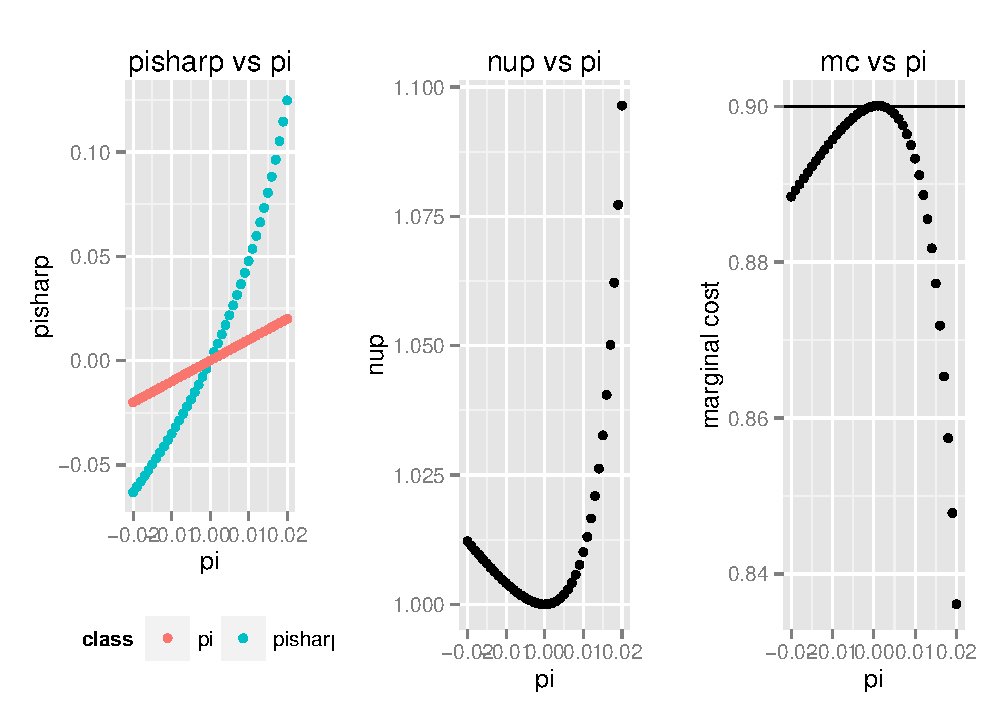
\includegraphics[width=0.8\textwidth]{Figures/R-simul-pi-pisharp-nup.pdf}
  \caption{数值模拟:$\{\pi^{\#},\nu^p\}$ vs $\pi$。模拟过程中设参数值$\phi=0.25$,$\epsilon=10$, $\beta = 0.99$。}
  \label{fig:simul-pi-pisharp-nup}
\end{figure}

给定$A=1$,工资决定式\eqref{eq:intm-prod-min-N-mc} $\Rightarrow$
\begin{equation}
  \label{eq:ss-wage}
  w = mc
\end{equation}
即工资等于劳动投入的边际成本。

式\eqref{eq:equili-agg-j-prod-DS} $\Rightarrow$ 边际产出$mpn$
\begin{equation}
  \label{eq:ss-mpn}
  mpn = \frac{1}{\nu^p}
\end{equation}
可见$\pi=0$时,mpn和mc的差距最小,体现为一个fixed price markup $\frac{\epsilon}{\epsilon -1}$。$\pi \neq 0$且越远离0时,经济体distorted的程度越大;此外,$\pi>0$时经济体的distorted程度,高于$\pi<0$时。

劳动力的供应式\eqref{HH-FOC-labor-supply} $\Rightarrow$
\begin{align*}
  \psi \cdot N^{\eta} &= C^{-\sigma} \cdot w \\
                      &= Y^{-\sigma} \cdot mc \\
                      &= \left(\frac{N}{\nu^p}\right)^{-\sigma} \cdot mc,
\end{align*}
整理得
\begin{equation}
  \label{eq:ss-labor-supply}
  N = \left[ \frac{1}{\psi} \cdot \left( \nu^p \right)^{\sigma} \cdot mc \right] ^{\frac{1}{\eta + \sigma}}
\end{equation}

总产出由式\eqref{eq:equili-agg-j-prod-DS}   \eqref{eq:ss-labor-supply}   \eqref{eq:ss-marginal-cost}得 $\Rightarrow$
\begin{align}
  \label{eq:ss-agg-output}
  Y &= \frac{N}{\nu^p},\nonumber \\
      &= \frac{\left[ \frac{1}{\psi} \cdot \left( \nu^p \right)^{\sigma} \cdot mc \right] ^{\frac{1}{\eta + \sigma}}}{\nu^p} \nonumber \\
      &= \left(\frac{1}{\psi}\right)^{\frac{1}{\sigma + \eta}} \cdot \left( v^p \right)^{-\frac{\eta}{\eta + \sigma}} \cdot
        \left[
        \frac{1-\phi \cdot \beta \cdot (1+\pi)^{\epsilon}}{1-\phi \cdot \beta \cdot (1+\pi)^{\epsilon-1}} \cdot \frac{1+\pi^{\#}}{1+\pi} \cdot \frac{\epsilon -1}{\epsilon}
        \right]^{\frac{1}{\eta + \sigma}}
\end{align}

\section{flexible price equilibrium 和 output gap}
\label{sec:flexible-price-output-gap}
\subsection{flexible price equilibrium}
\label{sec:flexible-price}

假定中间产品生产者可以自由调整价格,对应$\phi = 0$。将变量加上角标$f$以标注。此时$\pi = \pi^{\#}$,且名义价格不会对实际变量产生任何影响。

Flexible price dispersion index式\eqref{eq:price-dispersion-index-noj} $\Rightarrow$
\begin{equation}
  \label{eq:flexible-price-dispersion-index}
  v_t^{p,f} = 1,
\end{equation}
即包括最终产品和中间产品在内的全部生产者都会采取同样的产品定价策略,使price dispersion位于最低值1。

Reset price inflation 式\eqref{eq:intm-update-inflation-aux} $\Rightarrow$
\begin{equation}
  \label{eq:flexible-price-marg-cost}
  mc_t^f = \frac{\epsilon - 1}{\epsilon},
\end{equation}
可见边际成本是price markup的倒数。企业的定价策略在于:给$mc$加上一个固定的fixed price markup权数,作为产品售价。

Flexible price wage $\Rightarrow$
\begin{align*}
  mpn_t^f &= \frac{\partial Y_t^f}{\partial N_t^f} = A_t, \\
  P_t^f &= mc_t^f \cdot \frac{\epsilon}{\epsilon-1},\\
  mc_t^f &= w_t,\\
  mpn_t &= p_t^f,
\end{align*}
整理得
\begin{equation}
  \label{eq:flexible-price-wage}
  w_t^f = A_t \cdot \frac{\epsilon-1}{\epsilon}.
\end{equation}

Flexible price labor supply $\Rightarrow$
\begin{align*}
  \psi (N_t^f)^{\eta} &= (C_t^f)^{-\sigma} \cdot w_t^f,\\
                      &=(Y_t^f)^{-\sigma} \cdot mc_t^f,\\
                      &=\left( A_t \cdot N_t^f \right)^{-\sigma} \cdot \left( \frac{\epsilon -1}{\epsilon} \cdot A_t\right),
\end{align*}
整理得
\begin{equation}
  \label{eq:flexible-price-labor-supply}
  N_t^f = \left(\frac{1}{\psi} \cdot \frac{\epsilon -1}{\epsilon} \cdot A_t^{1-\sigma}\right)^{\frac{1}{\sigma + \eta}}.
\end{equation}

Flexible price aggregate output $\Rightarrow $
\begin{equation}
  \label{eq:flexible-price-agg-output}
  Y_t^f = A_t \cdot N_t^f = \left(\frac{1}{\psi} \cdot \frac{\epsilon -1}{\epsilon}\right)^{\frac{1}{\sigma + \eta}} \cdot  A_t^{\frac{1+\eta}{\sigma + \eta}}
\end{equation}

可见flexible price $(\phi =0)$情况下,名义波动不会对真实变量产生影响。

\subsection{output gap}
\label{output-gap}
定义output gap $\ln X_t \equiv \ln Y_t - \ln Y_t^f$,表示flexible price $(\phi = 0)$情况下产出$Y_t^f$与sticky price $(\phi >0)$情况下产出$Y_t$的差。

稳定状态下,$Y^f$的值由式\eqref{eq:flexible-price-agg-output}给出;
\begin{equation*}
%\label{ss-flexible-price-agg-output}
    Y^f = \left(\frac{1}{\psi} \cdot \frac{\epsilon -1}{\epsilon}\right)^{\frac{1}{\sigma + \eta}}
\end{equation*}

由此可得稳态output gap的值:
\begin{equation}
  \label{eq:ss-output-gap}
  \frac{Y}{Y^f} =
  \left[
    \frac{1-\phi \cdot \beta \cdot (1+\pi)^{\epsilon}}{1-\phi \cdot \beta \cdot (1+\pi)^{\epsilon -1}} \cdot \frac{1+\pi^{\#}}{1+\pi}
  \right]^{\frac{1}{\eta + \sigma}} \cdot
  \left(
    \nu^p
  \right)^{- \frac{\eta}{\eta + \sigma}}
\end{equation}
output gap的性质,分两种情况来讨论:

\begin{enumerate}
\item $\pi = 0$ $\Rightarrow$ $\pi^{\#} = \pi = 0$,$\nu^p = 1$ $\Rightarrow$ $Y=Y^f$ $\Rightarrow$ $\ln X = 0$,
\item $\pi >0$ $\Rightarrow$ $\pi^{\#} > \pi$, $\nu^p >1$ $\Rightarrow$ $Y<Y^f$ $\Rightarrow$ $\ln X < 0$。
\end{enumerate}
即在sticky price $(\phi >0)$条件下,稳态的output gap(对数)为负。


\section{Taylor法则}
\label{seq:Taylor-Rule}
假定中央银行的货币政策着眼于利率而非货币供应量:通过盯紧通货膨胀和产出这两个变量,灵活制定内生的货币政策以达到既定的利率目标\footnote{膏按:外生利率政策会导致indeterminacy问题,补充一个Appendix。}。常见的内生货币政策如Taylor法则:

\begin{equation}
  \label{eq:MP-Taylor-Rule}
  (i_t-i) = \rho_i \cdot (i_{t-1}-i) + (1-\rho_i) \cdot i+ (1-\rho_i) \cdot \left[
    \theta_{\pi} \cdot (\pi_t - \pi) + \theta_{x} \cdot (\ln X_t - \ln X)
  \right] + \varepsilon_{i,t},
\end{equation}
其中$i_t$表示名义利率。$X_t$表示output gap,见第\ref{output-gap}节。去掉下角标的变量表示其稳态值。$0 \le \rho_i \le 1$表示smoothing parameter。$\theta_\pi \ge 0$,$\theta_{x} \ge 0$。外生利率冲击$E\{ \varepsilon_{i,t}\} = 0$。

不难看出式\eqref{eq:MP-Taylor-Rule}的Taylor法则是个局部调整的货币政策:如果将稳态值$i$和$\pi$视作长期目标,则中央银行根据上期名义利率(距其稳态值)的偏离程度,以及当前期目标值(距其稳态值)的偏离程度,来灵活调整当期的名义利率;当前期目标值包括通货膨胀和output gap。一旦当期名义利率的调整目标确定,中央银行即通过向市场印发货币等手段,调节市场上的货币量,来实现其名义利率的目标。

\section{完整的均衡条件}
\label{sec:full-set-equilibrium-conditions}
经济系统的均衡解包括下述12个变量$\{ C_t, N_t, w_t, mc_t, Y_t, v^p_t, i_t, \pi_t, \pi^{\#}_t, x_{1,t}, x_{2,t}, A_t \}$,以及12个等式:

跨期消费的Euler equation 式\eqref{HH-FOC-euler-consumption} $\Rightarrow$
\begin{equation*}
    C_t^{-\sigma} = \beta \cdot E_t\{ C_{t+1}^{-\sigma} \cdot (1+i_t) \cdot \frac{P_t}{P_{t+1}}\}=\beta \cdot E_t\{ C_{t+1}^{-\sigma} \cdot (1+i_t) \cdot ( 1+\pi_{t+1} )^{-1}\}.
\end{equation*}

劳动力供应式\eqref{HH-FOC-labor-supply} $\Rightarrow$
\begin{equation*}
    \psi \cdot N_t^{\eta} = C_t^{-\sigma} \cdot w_t.
\end{equation*}

工资/边际成本的决定式\eqref{eq:intm-prod-min-N-mc} $\Rightarrow$
\begin{equation*}
    mc_t = \frac{MC_t}{P_t} = \frac{W_t}{A_t \cdot P_t} = \frac{w_t}{A_t}.
\end{equation*}

总消费与总产出的关系式\eqref{eq:HH-problem-C-Y} $\Rightarrow$
\begin{equation*}
  C_t = Y_t.
\end{equation*}

总量生产函数式\eqref{eq:equili-agg-j-prod-DS} $\Rightarrow$
\begin{equation*}
  Y_t = \frac{A_t \cdot N_t}{\nu^p_t}.
\end{equation*}

Price dispersion index 式\eqref{eq:price-dispersion-index-noj} $\Rightarrow$
\begin{equation*}
  \nu^p_t = (1-\phi) \cdot (1+\pi^{\#}_t)^{-\epsilon} \cdot (1+\pi_t)^{\epsilon} + \phi \cdot (1+\pi_t)^{\epsilon} \cdot \nu^p_{t-1}.
\end{equation*}

Evolution of inflation 式\eqref{eq:agg-inflation-index} $\Rightarrow$
\begin{equation*}
    \left(1+\pi_t\right)^{1-\epsilon} = (1-\phi) \cdot \left(1+\pi^{\#}_t\right)^{1-\epsilon} + \phi.
\end{equation*}

Reset price inflation 式  \eqref{eq:intm-update-inflation-aux} $\Rightarrow$
\begin{equation*}
  (1+\pi^{\#}_t) = \frac{\epsilon}{\epsilon -1} \cdot \left( 1+\pi_t \right) \cdot \frac{x_{1,t}}{x_{2,t}}.
\end{equation*}

两个reset price inflation的辅助变量,式\eqref{auxiliary-X1}-\eqref{auxiliary-X2} $\Rightarrow$
\begin{align*}
  x_{1,t} &\equiv C_t^{-\sigma} \cdot Y_t \cdot mc_t + \beta \cdot \phi \cdot E_t \left(1+\pi_{t+1} \right)^{\epsilon} \cdot x_{1,t+1},\\
  x_{2,t} &\equiv C_t^{-\sigma} \cdot Y_t + \beta \cdot \phi \cdot E_t \left( 1+\pi_{t+1} \right)^{\epsilon -1} \cdot x_{2,t+1}.
\end{align*}

Taylor rule 式\eqref{eq:MP-Taylor-Rule} $\Rightarrow$
\begin{equation*}
  (i_t-i) = \rho_i \cdot (i_{t-1}-i) + (1-\rho_i) \cdot i+ (1-\rho_i) \cdot \left[
    \theta_{\pi} \cdot (\pi_t - \pi) + \theta_{x} \cdot (\ln X_t - \ln X)
  \right] + \varepsilon_{i,t}.
\end{equation*}

Exogenous productivity shock 式\eqref{eq:exo-prod-shock} $\Rightarrow$
\begin{equation*}
  \ln A_t = \rho_a \cdot \ln A_{t-1} + \varepsilon_{a,t} .
\end{equation*}

\section{对数线性化}
\label{sec:BNK-log-lin-system}
\subsection{对数线性化计算}
\label{sec:BNK-log-linearization}
求解上述均衡方程组,方法之一是利用Dynare等计算机软件进行计算。此外,在模型较简单的情况下,也可以围绕zero-inflation steady state $\pi=0$的点,手算对数线性化的近似。

Euler equation 式\eqref{HH-FOC-euler-consumption} + 式\eqref{eq:HH-problem-C-Y} $\Rightarrow$
\begin{equation*}
  -\sigma \cdot \ln Y_t = \ln \beta - \sigma E_t \ln Y_{t+1} + i_t - E_t \pi_{t+1},
\end{equation*}
设$\ln (1+i_t) \approx i_t$,$\ln (1+\pi_t) \approx \pi_t$。将上式中每个变量分别围绕自己的稳态值作一阶泰勒级数展开,
\begin{equation*}
  -\sigma \cdot \frac{Y_t - Y}{Y} = -\sigma \cdot E_t \frac{Y_{t+1} - Y}{Y} + (i_t - i) - E_t (\pi_{t+1} - \pi),
\end{equation*}
定义$\tilde{Z}_t \equiv (Z_t - Z)/Z$作为变量$Z_t$距离其稳态值$Z$的偏离程度,$Z_t=(Y_t,N_t,A_t,\ldots)$;为了手算方便,对于已经是rate form的变量,包括利率$i_t$、通货膨胀率$\pi_t$和$\pi^{\#}_t$、price dispersion index $v^p_{t}$,直接用差分代替增速形式,如$\tilde{i}_t \equiv i_t -i$。上式进一步改写为
\begin{equation}
  \label{eq:log-lin-euler}
  \tilde{Y}_t = E_t \tilde{Y}_{t+1} - \frac{1}{\sigma} \left[\tilde{i}_t - E_t \tilde{\pi}_{t+1}\right].
\end{equation}

式\eqref{eq:log-lin-euler}又被称为New Keynesian IS Curve (NKIS)。Keynesian IS curve反映了投资(Investment)和投资(Saving)之间的对应关系。这里的“基础”New Keynesian模型中并未考虑投资,它反映了当期消费需求和实际之间的负相关关系。与传统IS curve相比,NKIS的“新”体现在其forward-looking的特征上:当期需求$(\tilde{C}_t = \tilde{Y}_t)$不只取决于实际利率$(\tilde{i}_t - E_t \tilde{\pi}_{t+1})$且负相关,还取决于对未来收入(消费)的期望$E_{t} \tilde {Y}_{t+1}$且负相关。

边际成本与工资的关系式\eqref{eq:intm-prod-min-N-mc} $\Rightarrow$
\begin{align}
  \tilde{mc}_t = \tilde{w}_t - \tilde{A}_t.
\end{align}

Price dispersion index 式\eqref{eq:price-dispersion-index-noj} $\Rightarrow$
\begin{align}
\label{eq:log-lin-price-dispersion-index}
  \tilde{\nu}^p_t &= \left[(-\epsilon) \cdot (1-\phi) \cdot (1+\pi^{\#})^{-\epsilon -1} \cdot (1+\pi)^{\epsilon}\right] \cdot (\pi^{\#}_t - \pi^{\#}) \nonumber\\
                    &+ \left[ \epsilon \cdot (1-\phi) \cdot (1+\pi^{\#})^{-\epsilon} \cdot (1+\pi)^{\epsilon -1} \right] \cdot \pi_t \nonumber\\
                    &+\left[ \epsilon \cdot \phi \cdot (1+\pi)^{\epsilon -1} \cdot \nu^p \right] \cdot (\pi_t - \pi) \nonumber\\
                    &+\left[ \phi \cdot (1+\pi)^{\epsilon} \right] \cdot \left(\nu^p_{t-1} - \nu^p \right) \nonumber\\
                  &=-\epsilon \cdot (1-\phi) \cdot \tilde{\pi}^{\#}_t + \epsilon \cdot (1-\phi) \cdot \tilde{\pi}_t + \epsilon \cdot \phi \cdot \tilde{\pi}_t + \phi \cdot \tilde{\nu}^p_{t-1} \nonumber\\
                    &=-\epsilon \cdot (1-\phi) \cdot \tilde{\pi}^{\#}_t + \epsilon \cdot \tilde{\pi}_t + \phi \cdot \tilde{\nu}^p_{t-1},
\end{align}
其中第三个等号用到$\pi = \pi^{\#} = 0$的假设条件。


Evolution of inflation 式\eqref{eq:agg-inflation-index} $\Rightarrow$
\begin{equation*}
  (1-\epsilon) \cdot \ln (1+\pi_t) = \ln \left[ (1-\phi) \cdot \left(1+\pi^{\#}_t\right)^{1-\epsilon} + \phi \right],
\end{equation*}
\begin{equation*}
  (1-\epsilon) \cdot (\pi_t - \pi) =
  \left[
    (1-\phi) \cdot (1-\epsilon) \cdot \left( 1+\phi^{\#} \right)^{-\epsilon} \cdot (1+\pi)^{\epsilon -1}
  \right],
\end{equation*}
\begin{equation}
  \label{log-lin-evolution-inflation}
  \tilde{\pi}_t = (1-\phi) \cdot \tilde{\pi}^{\#}_t.
\end{equation}

由式\eqref{log-lin-evolution-inflation}可见,actual inflation和reset price inflation呈一定比例变化,比例$1-\phi$为全部企业中,调整价格者所占的比重。

总量生产函数式\eqref{eq:equili-agg-j-prod-DS} $\Rightarrow$
\begin{align}
  \label{eq:log-lin-agg-prod-func}
  \tilde{Y}_t &= \tilde{A}_t + \tilde{N}_t - \tilde{\nu}^p_t \nonumber \\
              &=\tilde{A}_t + \tilde{N}_t - \left[\epsilon \cdot \tilde{\pi}_t -\epsilon \cdot (1-\phi) \cdot \tilde{\pi}^{\#}_t + \phi \cdot \tilde{\nu}^p_{t-1}\right]\nonumber \\
              &\approx \tilde{A}_t + \tilde{N}_t,
\end{align}
第三行的约等号是由于,从式\eqref{eq:log-lin-price-dispersion-index}可得,在zero inflation steady state下,$\pi=\pi^{\#}=0$且$\nu^p=1$,则$(\nu^p_t-1) = \phi \cdot (\nu^p_{t-1}-1)$。这说明$\tilde{\nu}^p_t=0$ $\forall t$。换句话说,在price dispersion index是一个二阶量;在我们围绕zero inflation steady state作一阶线性近似时,可以省略。

flexible price下的产出水平式\eqref{eq:flexible-price-agg-output} $\Rightarrow$
\begin{equation}
  \label{eq:log-lin-flexible-price-output}
  \tilde{Y}_t^f = \frac{1+\eta}{\sigma + \eta} \cdot \tilde{A}_t.
\end{equation}

劳动力供应式\eqref{HH-FOC-labor-supply} $\Rightarrow$
\begin{align*}
%\label{log-lin-labor-supply}
    \eta \cdot \tilde{N}_t &= -\sigma \cdot \tilde{Y}_t + \tilde{w}_t \nonumber \\
                           &= -\sigma \cdot \tilde{Y}_t + \tilde{mc}_t + \tilde{A}_t,
\end{align*}
引入式\eqref{eq:log-lin-agg-prod-func}替代LHS的$\tilde{N}_t$,引入式\eqref{eq:flexible-price-agg-output}替代RHS的$\tilde{A}_t$,可得
\begin{align}
  \label{eq:log-lin-labor-supply}
  \tilde{mc}_t &= \left(\sigma + \eta \right) \cdot \tilde{Y}_t - (1+\eta) \cdot \tilde{A}_t \nonumber \\
               &= (\sigma + \eta) \cdot \tilde{Y}_t - \left(\frac{\sigma + \eta}{1+\eta} \right) \cdot \tilde{Y}^f_t \cdot (1+\eta)\nonumber \\
               &= (\sigma + \eta) \cdot \left(\tilde{Y}_t - \tilde{Y}^f_t \right) \nonumber \\
               &= (\sigma + \eta) \cdot \tilde{X}_t,
\end{align}
式\eqref{eq:log-lin-labor-supply} LHS是fixed steady state price markup的倒数$(\epsilon - 1 )/\epsilon$。
\begin{enumerate}
\item $\tilde{X}_t = 0$ $\Rightarrow$ $\tilde{mc}_t = 0$ $\Rightarrow$ $mc_t \equiv mc = \frac{\epsilon-1}{\epsilon}$ $\Rightarrow$ price markups等于desired steady state fixed price markup $\frac{\epsilon}{\epsilon -1}$
\item $\tilde{X}_t <0$ $\Rightarrow$ $Y_t < Y_t^f$ $\Rightarrow$ $\tilde{mc}_t < mc$ $\Rightarrow$ 实际边际成本小于steady state fixed price markup, $mc_t < \frac{\epsilon}{\epsilon -1}$ $\Rightarrow$ 该经济体 is more distorted。
\end{enumerate}

辅助变量$x_{1,t}$式\eqref{auxiliary-X1} $\Rightarrow$
\begin{equation*}
  \ln x_{1,t} = \ln \left[ Y_t^{1-\sigma} \cdot mc_t + \phi \cdot \beta \cdot E_t \cdot (1+\pi_{t+1})^{\epsilon} \cdot x_{1,t+1}\right],
\end{equation*}
\begin{align}
\label{log-lin-X1-step1}
  \frac{x_{1,t} - x_{1}}{x_1} &= \frac{1}{x_1} \cdot \{ \left[(1-\sigma) \cdot Y^{-\sigma} \cdot mc \right]\cdot (Y_t - Y) \nonumber\\
                              &+Y^{1-\sigma} \cdot (mc_t - mc) \nonumber\\
                              &+\left[\phi \cdot \beta \cdot \epsilon \cdot (1+\pi)^{\epsilon -1} \cdot x_1\right] \cdot E_t (\pi_{t+1}-\pi)\nonumber\\
                              &+\left[ \phi \cdot \beta \cdot (1+\pi)^{\epsilon}\right] \cdot E_t (x_{1,t+1} - x_1) \},
\end{align}
由式\eqref{auxiliary-X1}可得,在$\pi = 0$时
\begin{equation}
\label{log-lin-X1-step2}
  x_{1} = \frac{Y^{-\sigma} \cdot mc}{1-\phi \cdot \beta},
\end{equation}
联立\eqref{log-lin-X1-step1}-\eqref{log-lin-X1-step2}得
\begin{equation}
\label{log-lin-X1-step3}
  \tilde{x}_{1,t} = (1-\sigma) \cdot (1-\phi \cdot \beta) \cdot \tilde{Y}_t + (1-\phi \cdot \beta) \cdot \tilde{mc}_t + \epsilon \cdot \phi \cdot \beta \cdot E_t \tilde{\pi}_{t+1} + \phi \cdot \beta \cdot E_t \tilde{x}_{1,t+1}.
\end{equation}

辅助变量$x_{2,t}$式\eqref{auxiliary-X2} $\Rightarrow$
\begin{equation*}
  \ln x_{2,t} = \ln \left[Y_t^{1-\sigma} + \phi \cdot \beta \cdot E_t \left(1+\pi_{t+1}\right)^{\epsilon -1} \cdot x_{2,t+1}\right],
\end{equation*}
\begin{align}
\label{eq:log-lin-X2-step1}
  \frac{x_{2,t}-x_2}{x_2} &= \frac{1}{x_2} \cdot \{ \left[(1-\sigma) \cdot Y^{-\sigma}\right] \cdot (Y_t - Y)\nonumber\\
                          &+\left[\phi \cdot \beta \cdot E_t (\epsilon -1) \cdot (1+\pi)^{\epsilon -2} \cdot x_2\right] \cdot (\pi_{t+1} - \pi)\nonumber\\
                          &+\left[\phi \cdot \beta \cdot E_t (1+\pi)^{\epsilon -1} \right] \cdot \left( x_{2,t+1} - x_2\right),
\end{align}
由式\eqref{auxiliary-X2}可得,在$\pi = 0$时
\begin{equation}
  \label{eq:log-lin-X2-step2}
  x_2 = \frac{Y^{-\sigma}}{1-\phi \cdot \beta}
\end{equation}

联立式\eqref{eq:log-lin-X2-step1}-\eqref{eq:log-lin-X2-step2}得
\begin{equation}
  \label{eq:log-lin-X2-step3}
  \tilde{x}_{2,t} = (1-\sigma) \cdot (1-\phi \cdot \beta) \cdot \tilde{Y}_t+ (\epsilon - 1) \cdot \phi \cdot \beta \cdot E_t \tilde{\pi}_{t+1} + \phi \cdot \beta \cdot E_t \tilde{x}_{2,t+1}.
\end{equation}

将式\eqref{eq:log-lin-X2-step3}-\eqref{eq:log-lin-X2-step3}代入式\eqref{eq:intm-update-inflation-aux}得
\begin{align}
\label{log-lin-reset-price-inflation-step1}
  \tilde{\pi}^{\#}_t - \tilde{\pi}_t &= \tilde{x}_{1,t}-\tilde{x}_{2,t} \nonumber \\
                     &=(1-\phi \cdot \beta) \cdot \tilde{mc}_t + \phi \cdot \beta \cdot E_t \tilde{\pi}_{t+1} + \phi \cdot \beta \cdot E_t \left(\tilde{x}_{1,t+1} - \tilde{x}_{2,t+1} \right).
\end{align}

式\eqref{log-lin-evolution-inflation}与\eqref{log-lin-reset-price-inflation-step1}联立,可得 Reset price inflation式
\begin{equation}
  \label{eq:log-lin-reset-price-inflation-mc}
  \tilde{\pi}_t = \left(\frac{1-\phi}{\phi}\right) \cdot (1-\phi \cdot \beta) \cdot \tilde{mc}_{t} + \beta \cdot E_t \tilde{\pi}_{t+1}.
\end{equation}

式\eqref{eq:log-lin-reset-price-inflation-mc}又被称为New Keynesian Philips Curve (NKPC),它反映了中央银行对产出和通货膨胀的trade off。也可以用式\eqref{eq:log-lin-labor-supply}中的output gap $\tilde{X}_t$代替边际成本$mc_{t}$,NKPC改写为
\begin{align}
  \label{eq:log-lin-reset-price-inflation-gap}
  \tilde{\pi}_t &= \left(\frac{1-\phi}{\phi}\right) \cdot (1-\phi \cdot \beta) \cdot \left[(\sigma + \eta) \cdot \left(\tilde{Y}_t - \tilde{Y}_t^f \right)\right] + \beta \cdot E_t \tilde{\pi}_{t+1}\nonumber \\
                &= \left(\frac{1-\phi}{\phi}\right) \cdot (1-\phi \cdot \beta) \cdot \left[(\sigma + \eta) \cdot \tilde{X}_t \right] + \beta \cdot E_t \tilde{\pi}_{t+1}.
\end{align}

或者,around a zero inflation steady state,用forward-looking形式表现NKPC
\begin{align}
  \label{eq:log-lin-reset-price-inflation-4ward-mc}
  \tilde{\pi_t} &= \left(\frac{1-\phi}{\phi}\right) \cdot (1-\phi \cdot \beta) \cdot \sum_{s=0}^{\infty} \beta^s \cdot \tilde{mc}_{t+s} \\
  \label{eq:log-lin-reset-price-inflation-4ward-gap}
                &= \left(\frac{1-\phi}{\phi}\right) \cdot (1-\phi \cdot \beta) \cdot (\sigma +\eta) \cdot \sum_{s=0}^{\infty} \beta^s \cdot \tilde{X}_{t+s}.
\end{align}

Keynesian PC curve 反映了通货膨胀率和边际成本之间的对应关系。NKPC的“新”体现在其forward-looking的特征上。  式\eqref{eq:log-lin-reset-price-inflation-4ward-mc}表明当前通货膨胀率和对未来实际边际成本的贴现值之间呈等比关系,边际成本表现为price markup的倒数。在价格是完全浮动的情况下$\phi = 0$,企业会根据desired constant markups给产品定价;如果企业预期未来的边际成本会增加,那么在定价时就会相应调低price markups。在存在价格粘性的情况下$\phi >0$,有机会在当前$t$期调整价格的企业,便会提前提高产品价格(以避免在未来$t+s$时间期内无法再次调整产品售价),以达到他们的desired price markup,这造成了通货膨胀。反之亦然。

NKPC curve的“斜率”与$\phi$负相关。随着$\phi$逐渐降低,NKPC线越来越陡峭。当$\phi \rightarrow 0$时,perfectly flexible price,NKPC线完全垂直,此时$\tilde{Y}_t = \tilde{Y}_t^f$,$\tilde{mc}_t = 0$。

Exogenous productivity shock 式\eqref{eq:exo-prod-shock} $\Rightarrow$
\begin{equation}
  \label{eq:log-lin-prod-shock}
  \tilde{A}_t =\rho_a \cdot \tilde{A}_{t-1} + \varepsilon_{a,t}.
\end{equation}

Taylor rule 式\eqref{eq:MP-Taylor-Rule} $\Rightarrow$
\begin{equation}
  \label{eq:log-lin-tayl-rule}
  \tilde{i}_t = \rho_i \cdot \tilde{i}_{t-1} + (1-\rho_i) \cdot \left[\phi_{\pi} \cdot \tilde{\pi}_t + \phi_{x} \cdot \tilde{X}_t \right].
\end{equation}

\subsection{线性模型}
\label{sec:BNK-log-linearization-system}
作线性近似处理后的经济系统,表述为如下5个变量$\left(\tilde{Y}_t, \tilde{i}_t, \tilde{\pi}_t, \tilde{Y}_t^f, \tilde{A}_t\right)$,5个等式
线性Euler equation,反映总量需求的NKIS式\eqref{eq:log-lin-euler} $\Rightarrow$
\begin{equation*}
  \tilde{Y}_t = E_t \tilde{Y}_{t+1} - \frac{1}{\sigma} \left(\tilde{i}_t - E_t \tilde{\pi}_{t+1}\right).
\end{equation*}

反映总量供应的NKPC式\eqref{eq:log-lin-reset-price-inflation-mc}或  \eqref{eq:log-lin-reset-price-inflation-gap} $\Rightarrow$
\begin{align*}
  \tilde{\pi}_t &= \left(\frac{1-\phi}{\phi}\right) \cdot (1-\phi \cdot \beta) \cdot \tilde{mc}_{t} + \beta \cdot E_t \tilde{\pi}_{t+1}\\
                &=\left(\frac{1-\phi}{\phi}\right) \cdot (1-\phi \cdot \beta) \cdot \left[(\sigma + \eta) \cdot \tilde{X}_t \right] + \beta \cdot E_t \tilde{\pi}_{t+1}.
\end{align*}

辅助变量,反映flexible price下的产出水平,式\eqref{eq:log-lin-flexible-price-output} $\Rightarrow$
\begin{equation*}
  \tilde{Y}_t^f = \frac{1+\eta}{\sigma + \eta} \cdot \tilde{A}_t.
\end{equation*}

Exogenous productivity shock 式\eqref{eq:exo-prod-shock} $\Rightarrow$
\begin{equation*}
  \tilde{A}_t =\rho_a \cdot \tilde{A}_{t-1} + \varepsilon_{a,t}.
\end{equation*}

反映货币政策的Taylor rule 式\eqref{eq:MP-Taylor-Rule} $\Rightarrow$
\begin{equation*}
  \tilde{i}_t = \rho_i \cdot \tilde{i}_{t-1} + (1-\rho_i) \cdot \left[\phi_{\pi} \cdot \tilde{\pi}_t + \phi_{x} \cdot \tilde{X}_t \right].
\end{equation*}
